\section{Simulating Users}

We will need to be able to simulate users and their preferences in order to quantify how well this algorithm is likely to work in production. We will make use of the ADS-16 Computational Advertising Dataset\cite{ads16} for this task. This dataset contains (amongst other things) a set of answers given by 120 users to 10 personality questions. The answers are given on a scale from -2 to 2 (inclusive of both ends). Each user's age, income bracket, and gender are also included. In addition, the dataset contains a set of 300 advertisements split evenly into 20 categories. Crucially, this dataset also provides a rating from 1 to 5 (inclusive of both ends) that each user gave to each ad.

We propose a method for modelling the relationship between the user data described above (the user's answers to the personality questions, age, income bracket, and gender) and that user's rating for a given ad. We will then generate a set of simulated users, and we will use this model to determine their interaction with ads.

Note that it is not important for our purposes what the personality questions specifically are --- only that their answers hold some predictive power with respect to the ad ratings.

The technique laid out in this section can be easily adjusted to work with a different (perhaps custom) dataset, as long as it contains data from which a simulated user can be generated, and their interaction with ads modelled.

For the sake of clarity, we will define the following terms for the data we have available to us:

\begin{gloss}
    b_{i,j} &= \textrm{user $i$'s answer to personality question $j$} \\
    &\in [-2,2] \cap \mathbb{Z} \\ \\
    g_i &= \textrm{user $i$'s gender} \\
    &\in [0,1] \\ \\
    a_i &= \textrm{user $i$'s age in years} \\
    &\in \mathbb{N} \\ \\
    \lambda_i &= \textrm{user $i$'s income bracket} \\
    &\in [0,3] \cap \mathbb{Z} \\ \\
    r_{i,k} &= \textrm{user $i$'s rating for ad $k$} \\
    &\in [1,5] \cap \mathbb{Z} \\ \\
    c_k &= \textrm{category of ad $k$} \\
    &\in [0,20) \cap \mathbb{Z} \\ \\
    \bar{r}_{i,c} &= \textrm{mean rating from user $i$ across all ads with category $c$} \\
    &= \textrm{mean}\left(\left\{ r_{i,k} | c_k = k \right\}\right)
\end{gloss}

With respect to $g_i$, we use a value of 1 to correspond to female, and 0 to male, though this is arbitrary. Furthermore, the dataset we are using only contains males and females, but this technique generalises seamlessly to non-binary identities corresponding to values in the range $(0,1)$.

For each user we construct a ``raw'' user feature vector $f'_i$ to encapsulate all of the user data we might use to predict $r_{i,k}$.

\begin{equation*}
    f'_i = \begin{bmatrix}
        b_{i,0} &
        \hdots &
        b_{i,9} &
        g_i &
        a_i &
        \lambda_i &
        \bar{r}_{i,0} &
        \hdots &
        \bar{r}_{i,19}
    \end{bmatrix}
\end{equation*}

We refer to this as a ``raw'' vector because it requires some processing to become useful. Our hope is to eventually simulate users, and this will involve sampling feature vectors from some known distribution. However, although the empirical distribution of each individual element can be found directly in our dataset, these features are not independent, and so cannot be sampled independently. This makes intuitive sense, as we might expect, for example, age to correlate with income bracket, but this intuition can be confirmed by inspecting the correlation matrix of these features across all users.

\begin{figure}[H]
    \centering
    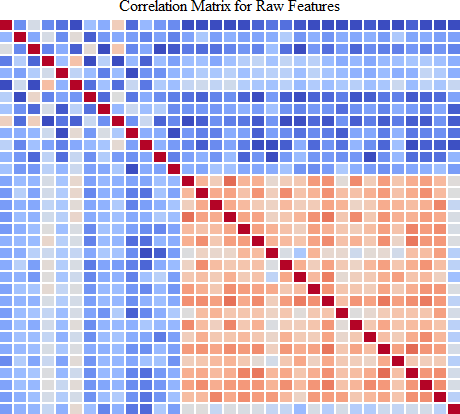
\includegraphics[width=0.6\textwidth]{raw_corr.png}
    \caption{Correlation matrix for components of $f'_i$}
\end{figure}

We therefore perform principal component analysis on these features, whose transform yields the user feature vectors $f_i\in \mathbb{R}^{33}$, whose components are all independent.

We assume that each of the components are normally distributed, and we can estimate the parameters of the distributions across all of the users in the dataset.

In addition to the data above, we also require the text present in each ad. With our dataset, we must rely on optical character recognition to extract the text from the image of each ads we are given. We then use a pre-trained GloVe\cite{glove} word embedding of dimension $d_e$ to embed each word of the ad.

This yields two tensors for the $k$\textsuperscript{th} ad, $\tensor*[_0]{v}{_k}$ and $\tensor*[_1]{v}{_k}$, which correspond to a one-hot vector encoding of $c_k$, and the ad's embedded word vectors respectively. The shape of $\tensor*[_0]{v}{_k}$ is $(20)$ and the shape of $\tensor*[_1]{v}{_k}$ is $(w_m, e_d)$ where $w_m$ is the maximum number of words in an ad.

We use a deep neural network including a transformer block\cite{transformer} generate an approximation $\hat{R}$ of the following function $R$:

\begin{equation*}
    R\left(f_i, \tensor*[_0]{v}{_k}, \tensor*[_1]{v}{_k}\right) = \textrm{onehot}\left(r_{i,k}\right)
\end{equation*}

such that

\begin{equation*}
    \textrm{argmax}\left(\hat{R}\left(f_i, \tensor*[_0]{v}{_k}, \tensor*[_1]{v}{_k}\right)\right) + 1 \approx r_{i,k}
\end{equation*}
The addition of 1 to the left hand side of the above is due to the fact that the indices of the one-hot vectors range from 0 to 4 (inclusive of both ends) whereas the values of $r_{i,k}$ range from 1 to 5 (inclusive of both ends).

The DNN has the following structure:

\begin{figure}[H]
    \centering
    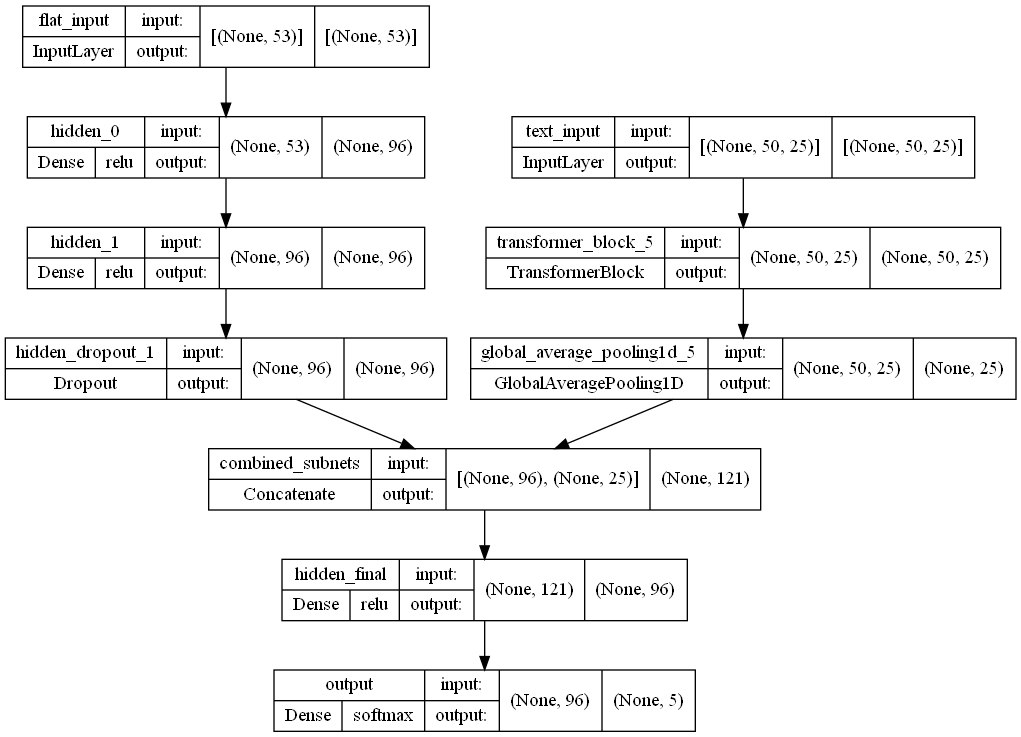
\includegraphics[width=0.9\textwidth]{sim_dnn.png}
    \caption{The structure of a DNN which approximates a given user's rating for a given ad, with $w_m=50$, $e_d=25$}
\end{figure}

The hyperparameters can be found in the appendix, and were determined using the Keras\cite{keras} implementation of the Hyperband algorithm\cite{hyperband}.